\subsection*{a}
Let us consider the two decays 
\begin{gather*}
    \tau^- \rightarrow \mu^- \, \bar\nu_{\mu} \, \nu_{\tau} \\
    \mu^- \rightarrow e^- \, \bar\nu_e \, \nu_{\mu}
\end{gather*}
represented by the two Feynman diagrams \\
\begin{figure}[hbtp]
    \centering
    \begin{minipage}{0.4\textwidth}
        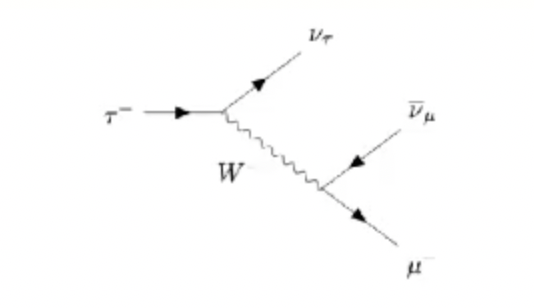
\includegraphics[scale=0.6]{ex4/tau.png}
        \caption{Feynman diagram for the reaction $\tau^- \rightarrow \mu^- \, \bar\nu_{\mu} \, \nu_{\tau}$}
    \end{minipage}
    \hfill
    \begin{minipage}{0.4\textwidth}
        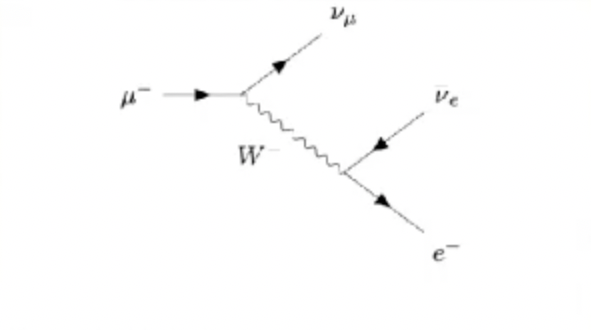
\includegraphics[scale=0.6]{ex4/mu.png}
        \caption{Feynman diagram for the reaction $\mu^- \rightarrow e^- \, \bar\nu_e \, \nu_{\mu}$}
    \end{minipage}
\end{figure}
The probability for a particle to get scattered by a certain potential is proportional to the squared of the so called \emph{amplitude} $\mathcal{M}$.
Assuming that the coupling constant $g^2$ of the Yukawa potential (atomic units)
\begin{equation*}
    V(r) = -\frac{g^2}{4\pi} \frac{e^{-r/R}}{r}
\end{equation*}
is small compared to $4\pi$ (this means that the potential can be considered as a perturbation to the free particle solution), then the amplitude $\mathcal{M}$ of the proces can be computed by means of the Born approximation
\begin{equation*}
    \mathcal{M}(\ve p) = \int V(\ve{r}) \, \exp(i\ve{r}\cdot\ve{r}) \, d^3\ve{r}
\end{equation*}
where $\ve{p} = \ve{p}_i - \ve{p}_f$ denotes the momentum difference between the initial and final state. By direct computation one can prove that 
\begin{equation}
    \mathcal{M}(\ve p) = \mathcal{M}(p^2) = - \frac{g^2}{p^2 + m_x^2}
    \label{eq:amplitude_born}
\end{equation}
where $m_x$ denotes the mass of the propagator. A multiplicative factor of $\sqrt{2}$ must be added if the spin interaction is taken into account. \\
In addition, the force carrier that governs the interaction is the $W$ boson, the mass of which is many times bigger than all the other involved masses. Hence a more suitable form of 
\ref{eq:amplitude_born} is 
\begin{equation*}
    \mathcal{M}(\ve p) = \mathcal{M}(p^2) = - \sqrt{2} \, \frac{g^2}{m_x^2} \approx 1.166 \cdot 10^{-5}~(GeV)^{-2} \equiv G_F
\end{equation*}
and $G_F$ is the Fermi coupling constant.
This results is known as \emph{leptons universality} and states that the amplitude of a lepton's decay process is a constant that does not depend on the chosen lepton. \\
At this point one can introduce the decay rate $\Gamma$ which is proportional to the probability of the process to occur
\begin{equation*}
    \Gamma \approx K M^2 A
\end{equation*}
where $A$ is a constant whose units are those of an energy to the fifth power, because $[M^2] = (GeV)^{-4}$. Since we expect the decay rate 
to depend on the generating particle, a reasonable choice for $A$ is $A=m_i^5$ where indeed $m_i$ denotes the mass of the generating particle. Hence
\begin{equation*}
    \Gamma \approx - \sqrt{2} K \, \frac{g^2}{m_x^2}m_i^5
\end{equation*}
Applying it to the particular case of the two given processes one obtains
\begin{equation}
    \frac{\Gamma\left(\tau^- \rightarrow \mu^- \, \bar\nu_{\mu} \, \nu_{\tau}\right)}{\Gamma\left( \mu^- \rightarrow e^- \, \bar\nu_e \, \nu_{\mu}\right)}
    \approx \left(\frac{m_{\tau}}{m_{\mu}}\right)^5 \approx 1.34 \cdot 10^6
    \label{eq:decay_widths_ratios}
\end{equation}

\subsection*{b}
The two relevant experimental quantities are the lifetime of the particles $\tau$ and the brancing ratios of the reactions. Let us define
$\Gamma_{\tau} \equiv \Gamma(\tau \to X \nu_{\tau})$ and $\Gamma_{\mu} \equiv \Gamma(\tau \to Y \nu_{\mu})$. Equation \ref{eq:decay_widths_ratios} 
can be rewritten as 
\begin{equation*}
    \frac{\Gamma\left(\tau^- \rightarrow \mu^- \, \bar\nu_{\mu} \, \nu_{\tau}\right)}{\Gamma\left( \mu^- \rightarrow e^- \, \bar\nu_e \, \nu_{\mu}\right)} =
    \frac{\Gamma\left(\tau^- \rightarrow \mu^- \, \bar\nu_{\mu} \, \nu_{\tau}\right)}{\Gamma_{\tau}} \
    \frac{\Gamma_\mu}{\Gamma\left( \mu^- \rightarrow e^- \, \bar\nu_e \, \nu_{\mu}\right)} \
    \frac{\Gamma_{\tau}}{\Gamma_{\mu}} = 
    \frac{B\left(\tau^- \rightarrow \mu^- \, \bar\nu_{\mu} \, \nu_{\tau}\right)}{B\left( \mu^- \rightarrow e^- \, \bar\nu_e \, \nu_{\mu}\right)} \ 
    \frac{\tau_{\mu}}{\tau_{\tau}}
\end{equation*}
which is a more relevant form for the experimental quantities.